\documentclass[12pt]{article}

\usepackage[margin= 1in]{geometry}
\usepackage{setspace}
\usepackage{amssymb}
\usepackage{amsmath}
\usepackage{mathptmx}
\usepackage{graphicx}
\graphicspath {{./images/}}

\doublespacing

\begin{document}
{\fontfamily{ptm} \selectfont


\begin{titlepage}
\vspace*{\fill}
\begin{center}
\Huge Extending ``Institutions, Human Capital, and Development"\\
\Large J Barnabas Lee\\
\small December 5, 2018
\end{center}
\vspace*{\fill}
\end{titlepage}

\section{Introduction}
\hspace{\parindent} One of the central quests of development economics is to identify the drivers of present economic development. In other words, the question remains: ``What are the fundamental causes of the
large differences in income per capita across countries?" This puzzle has led to examination of cases of ``miracle" growth such as the Asian Tigers, as compared to the struggling economies of the present.  Other literature has compared such ideas as the adoption trade policies and methods of industrialization such as ``Import- Substitution" versus ``Export-Led" to explain present growth levels. Daron Acemoglu, Simon Johnson, and James A. Robinson (2001) theorize that the institutions established during the colonial era have a direct effect on present institutions, which in turn have either hindered or driven economic success. This paper established that relative geographic location did not cause poorer economic performance. Rather, the harmful effects of colonization contributed to the struggles in the present day.

\begin{flushleft}
(Pot.) Settler Mortality $\rightarrow$ Settlements $\rightarrow$ Early Inst. $\rightarrow$ Current Inst. $\rightarrow$ Current Performance
\end{flushleft}

Using Acemoglu et al. (2001) as a backdrop, I will examine Daron Acemoglu, Francisco A. Gallego, and James A. Robinson's (2014) extension testing the robustness of the effect of institutions against estimates of the effect of human capital (HK). They find that the effect of human capital endowments by European colonists is overestimated. I believe that the authors overlooked the importance of geographic location as a contributing factor to a country's ability to utilize human capital endowments. This consideration would strengthen their argument if even the effect of this interaction were to be negligible.\\

This paper as well as my review of it contribute to the existing literature by emphasizing the importance of institutions. In terms of policy implications, while the intuition does not lend itself to any prescriptive predictions, provides a positive outlook for developing countries who have attempted at implementing growth-inducing institutions.\pagebreak

\section{Article Summary and Theory}

\hspace{\parindent} In this paper, I am extending, ``Institutions, Human Capital, and Development", Acemoglu, Gallego, and Robinson (2014) find that human capital endowments do not represent as large of an effect on present economic growth as other parts of the literature posit. They argue that assuming ``institutions and human capital as exogenous" leads to omitted variable bias and differential measurement error. With this in mind, they conclude that ``there is no support for the view that differences in human capital endowments of early European colonists have been a major factor" in economic development.  The impact of institutions is much stronger when controlled for, than the effects of human capital endowments. This means that countries with greater human capital endowments did not necessarily grow due to that advantage, but due to better institutions conducive to growth. Human capital would then be better developed regardless of the initial level endowed by the colonial power. These effects are seen by instrumenting human capital endowments, measured in years of schooling, with protestant missionary activity in a Two-Stage Least Squares regression.\\


Acemoglu et al. (2014) builds on the original model proposed by Acemoglu et al. (2001). The original logic is as follows: certain colonial territories had a higher probability of colonists dying, usually due to the pervasiveness of disease. So, if there was a high chance that a settler would die in a colony, the colonial power would choose to implement extractive institutions. Extractive policies focused on such areas as ``labor coercion such as slavery, monopolies, legal discrimination, and rules that made the property rights of the indigenous masses insecure". In territories that had a higher probability of survival, namely places with fewer diseases, the colonial power might choose to implement settlement institutions. In an attempt to replicate conditions and institutions from the home European countries, the settlers established inclusive institutions that helped economic growth. Extractive states are characterized by institutions that were conducive to extracting resources to remit back to the home country without provisions for institutions with respect to living in those colonies in the long-run. Settlement institutions established such ideas as intellectual property and rule of law, which incentivized and promoted economic growth. Ultimately, the effect of colonial institutions have proven to persist to the present, affect the country's current institutions.\\

The effects of human capital endowments, measured in years of schooling, is found by the instrument protestant missionary activity. The logic behind this instrument is that this activity helped to develop human capital through the development of people’s ability to read (presumably to be able to read the Bible). Acemoglu et al. find that when properly specified with institutions, the effect of human capital becomes very small, to the point that matches microeconomic (Mincerian) estimates. In fact, the authors go so far as to show that extractive colonies actually experienced higher levels of human capital endowment. This supports the original 2001 hypothesis about the effect of institutions being prime in the effects seen on present economic growth.\\

These tests are done in two contexts: cross-regional and cross-country. In the cross-country  context, the authors build on the 2001 paper to show that ``Protestant missionary activity was determined by idiosyncratic factors and need not be correlated with the potential for future economic development". The cross-regional context shows that while current human capital levels have significant effects on GDP growth, when human capital levels are instrumented for by missionary activity, the effect becomes insignificant. The ultimate conclusion, then, is that ``effects of human capital are cut down to the plausible range" when ``the fundamental cause of cross-country economic development, institutional differences, is controlled for".\pagebreak



\section{Analysis}

\subsection{Conceptual clarity}
		
The main causal variable is institutions, as outlined in Acemoglu et al.'s (2001) paper lays out. The authors define ``good" institutions as factors that incentivize investments in capital, both human and physical. The differences in income then between countries with ``good" capital come from the differences in ability to use those factors efficiently. While institutions are not explicitly defined in this paper, it is assumed to mean the factors used in production. Physical capital has a deterioration rate and is replaceable. Conceptually, physical capital should always be tangible in some way.\\

Human capital, which includes such factors as innovation and education, is one of the components of Total Factor Productivity (TFP) as defined by North and Thomas (1973) and the causal variable we are looking to find a null effect for. Rich countries are said to have higher levels of TFP, which also includes physical capital in the form of "machines, tools, and factories". However, this description is not implying a causal relationship but defines "what it means to be prosperous". Human capital is not simply a measure of the population as the sheer number of laborers in the work force is not part of the measure. But, the measure of a population's abilities IS an example of human capital.\\

The dependent variable then logically follows as GDP. In this case it is specified as GDP growth per capita with Purchasing Power Parity adjustment. This measure is a sum of the value of all the final goods and services transacted within a country per year. For this study, it is also standardized using Purchasing Power Parity. Essentially this means that country currencies are compared by the currency's ability to purchase a standard basic basket of goods. If two countries have equal currencies, then the basket of goods is priced the same in both countries. Per capita means that the GDP levels in each country are divided by the total population to find how much of the GDP is attributed to the average person.\\

All concepts seem to be fairly well defined within Acemoglu et al.'s (2014) paper. This is partly because the paper relies on many of the definitions and concepts from the earlier paper. I believe there are some measurement problems with the variables assigned. However, I will address those later.\\







\subsection{Theoretical coherence}


Ultimately, do institutions cause economic growth? This paper simply rules out human capital endowments as the primary cause and contributes to the literature by showing the minimal effects it has is actually counter to the broadly held intuitions of those making the argument for its importance. Human capital endowments, counter to what might be common intuition was more prevalent in countries with extractive institutions, which means that even if human capital were to have an effect, it would be a negative one as we already know the relationship between institutions and growth.\\

\subsection{Research design concerns or limitations}


The measurement validity concerns mostly lies in the idea of whether the measures for institutions seems legitimate. The authors use rule of law as their main institution variable. While this is a very important institution for the incentivizing of investment in capital, it does not have a direct effect on the economy. Now rule of law can expand to possibly include intellectual property laws, but that is just a subsection of the variable. It very well may be true that rule of law is the most quantifiable measure, and while it is not technically an instrument but a measurement, it is debatable whether it is the most relevant.\\

Human capital encapsulates the qualities of individuals in a group that contribute to the development of aggregate income. Acemoglu et al. refer to specific moments of human capital as proximate factors: innovation, education, and marginal propensity to save. These measurable yet intangible factors contribute greatly as factors of aggregate production. As this generates production, it aggregates to total income or GDP, in this case measured in GDP per capita PPP adjusted. Ultimately, does human capital play a role in economic growth? Most probably. However, what we are examining in this paper is whether human capital "given" by colonizing powers had the effect on institutions in the past, thus having its effects persist to the present. Human capital may seem like too abstract of a concept to measure, but while institutions are also a widely accepted source of economic growth, it has been more defined by specific measures. Instrumenting human capital endowment with missionary activity does not have enough of a direct effect on human capital development. The implication that protestant missionaries teaching how to read the colonizing language as a development is that the form of communication used in these regions previously are not valid. The reasoning must be carefully parsed out that the ability to read another language expanded the limits of interaction of people is the true reason why the missionary activity can measure the human capital endowments. The implications may contain negative and obsolete stereotypes that might not be worth exploring. Rather, I think if more specific measures of current human capital development indicators and tracking those back in time might be a more effective way of arguing current economic growth caused by human capital. This may have the additional added bonus of coming up with more robust results than Mincerian estimates.\\

Furthermore, the authors seem to have mostly used a joint method of Mill’s methods of agreement or difference. They are finding results of GDP and seeing the effects of one change in characteristics of the past (HK endowments). However, it also is attempting to show that countries with similar HK endowments don’t have a significant difference in GDP. Also, the study finds that institutions play a larger in role in current GDP by holding them the same and finding that HK does not play as significant role. This demonstrates that both agreement and difference methods were used.\\

The paper examines the effects of the causal variable on the dependent variable on two levels: both the cross-country and cross-regional levels. This allows for a more comprehensive understanding of the effect of institutions on economic growth. While GDP is measured on a per capita basis, it is not valid to say that each person accounts for that economic value. The aggregate is not a sum of the averages but the aggregate divided can be an average. In other words, the unit of analysis would be country and region in the two models, respectively. While human capital needs to be distributed among the population, it affects the whole country or region. Additionally, because institutions and the capital go hand in hand, it is most appropriate to aggregate the characteristics to the country or region.\\

This paper examines what can be considered a natural experiment. While there is undoubtedly some selection bias, such as which countries received human capital as selected by the colonizing powers, the effects remain, demonstrating how this can be seen as the effect of a treatment. The logic behind the colonizing powers is actually what is intuitively interesting anyway, so one would actually look for that selection bias so as to determine which factors really determined the economic growth factor roots. The study holds the property of as-if randomization. The treatment cannot be changed as it is in the past. Yet, the paper studies what can be considered a natural experiment. Nature decided which countries would have rampant disease and not. There was no synthetic control on which countries had coastline or had natural resources. But the results are as-if they are randomized because while not specifically manipulated with randomized treatment, it was decided by nature in a way of being random in itself.\\

The counterfactuals are not plausible due to the endogeneity and interconnected nature of the conceptual variables. Changing the level of human capital endowment in a country would be changing the very parameters that colonizing powers used decide how much to endow. This would change the very essence of the research question. \\

It is conceivable that colonized countries could have established policies and institutions as imitations or counters to surrounding former colonies based on their successes or failures. These policy choices may lead to better or worse outcomes, whether or not it is due to the different or same policies. The spillover effects of institutions may see a decrease in marginal benefit in comparison to the original country that established the policies. However, that logic would require the very first colony to establish settler institutions to have the highest growth rates which are not necessarily true. Rather, the spillover effects are often contained by the identity and livable conditions that contributed to settler mortality, as examined in this paper. \\

Additionally, when reasoned it makes sense that a colonizing power would have access to a finite amount of HK to endow meaning that if one colony received more endowments it could be taking away from another. The total amount of human capital endowment then is part of the same pot from each colonizing power. It would then follow that it would be interesting how the correlation between one colony's endowment versus another's.\\


While the measure for distance from the coast is used in the cross-regional analysis, there should be some similar measure in the cross-country analysis. Granted, distance from the coast is not an intuitive measure for a whole country. Rather, a measure such as total distance of coastline as a border for the country would be a useful measure. This variable probably has some correlation if not causation with the human capital endowments as the simple idea of physical access by colonizing powers can be found. Additionally, countries who have more coastline are probably better performers in today's economy due to the ability to have access to trade routes since the colonial era. Even if it were not ports, the coast has access to natural resources as well. This means that the intrinsic value of a body of water, especially one that was interconnected would confound the study.\\
 
It could be that there is an endogeneity issue for the cross-country analysis. When the dummies for colonizing power are put in, similar to the mention in the SUTVA section, there is a limited influence of each power. Restated, a colonizing power only had the means to settle a finite number of colonies which means that the intent to set up settlement colonies was affected by how many other settlements already existed. Additionally, the finite amount of human capital that was able to be endowed was probably finite for each colonizing power. This means that there are colliders in the paper that revolve around the basis that colonizing powers, while having much higher levels of human capital and physical capital, had finite numbers of people and endowable human capital. \\

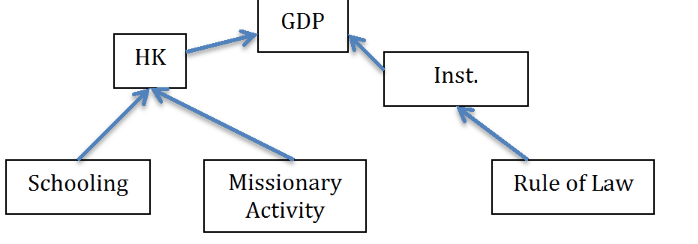
\includegraphics[scale = 1.25]{DAG}
Above is the DAG for the theory of this paper. Due to the endogeneity of human capital and institutions, the instruments were needed. In other words, the lowest level on the DAG actually represents instruments rather than a purely causal relationship. The main assertion is that institutions are the primary effect on GDP. While human capital, and its endowments also \\

The paper really only examines cross-sectional findings. This is due to the very nature of the question as the temporal aspect is already built into the model. It would be irresponsible to then call this any sort of time series study as it only looks at two time periods in which variables from both time periods are used to determine the causality. 
I don’t believe there are any extraneous variables. The DAG explains their main theory. However, later tables add in extra variables and controls, of which I am most interested in. Namely, the effects on institutions by factors such as settler mortality and population density are added later. Thanks to the two-step structure of this paper it allows for analysis with instrumental variables that make HK and institutions much more measurable.
The internal validity is probably fairly sound, seeing as this is a commonplace structure of question and investigation.
The authors mention that there is some selection bias as this question is limited to how former colonies have developed. This means that this theory doesn’t really apply to settings in which the country wasn’t’ colonized, or extracted from. Also, there is a skew in the number of observations with high versus low HK endowments. This means that the study is not generalizable to all countries and their ability to have high economic performance or, put simply, lacks external validity
 \\


Perhaps it is possible that ethnic fractionalization paired with selectorate theory meant that those countries with lower ethnic heterogeneity were more stable and experienced less war. This might allow for greater development of physical and human capital rather than the production of war. Ultimately, this could explain the difference in aggregate income in former-colonies. This also affects the ability of a colonizing power to be able to settle, as well as the its ability to endow human capital values. The specialization, slightly differing from the Guns-Butter tradeoff, allows for another factor that contributes to the accounting of settler mortality, but also the mortality of human capital even if the endowment was given.\\


\section{Suggested Extensions}

Extension 1: Add a variable for Present Population Density. (Cross-Country)

The basic Solow model of economic growth derives the intuition that population growth causes GDP growth by using a simple model of an economy in which the only inputs are Capital and Labor in a Cobb-Douglas form. When calculated at the Balanced Growth Path the model finds that GDP growth (total, not per capita) is equal to population growth.\\

\begin{equation}
\begin{split}
Y & = K^{\alpha}L^{1 - \alpha}\\
\hat Y  & =  \alpha K + (1 - \alpha) L\\
\hat L & = n\\
At \ Balanced \ Growth \ Path \ \hat Y & = \hat K \\
then \ (1 - \alpha)\hat Y & = (1 - \alpha) n\\
\hat Y & = n\\
\end{split}
\end{equation}

This would demonstrate another nail in the coffin of the basic Solow model and it's implication that population growth leads to overall GDP growth. Because a state's border's are relatively unchanged using historical data to match present delineations, the population density can be used as a total population measure. So, if present and past population densities are gathered, it can be used to create a population growth variable. If population growth and total GDP growth are not similar or even the same sign, it effectively demonstrates that while the Solow model was helpful for understanding GDP growth, it is not found in the empirics. The variable could also be a percent difference from 1900 to present, leading to possibly more accurate measures. The expectation is that there is no or insignificant effects on current economic performance by population growth. There are a number of population dynamics studies that may contain data to use for this extension. However, my main extension follows.\\

Extension 2:  Add an interaction term between inverse distance to coast and the human capital endowment (Cross-Regional)\\

This extension would be driven by the understanding that more than a human capital endowment, development was driven more by the ability to use such capital. I would argue that the further from the coast, the more the ability to use the human capital would be decreased. The logic would follow from the fact that trade centers were generally near if not directly on the coast. The situation of these centers would mean that regions far from the coast would have much less opportunity to use the human capital, much less develop it to levels in which it could match the regions on the coast. Additionally, state capitals were more than likely social or cultural centers where human capital might have found its greatest utility. Since social and cultural centers usually doubled as economic centers, the intuition continues. Also, the further inland a region was, the less likely it was that settlement institutions were established there. Intuitively then, the further inland a region was, the less likely it is to have consistently positive growth rates, a generally accepted notion. However, the causal logic is what leads us to this conclusion. Being inland would mean that human capital, even if heavily endowed, would not be used well and therefore not help in generating economic growth. As mentioned above, it might be possible to run this through the cross-country model as well. There may be too large of an effect than what is expected. The general expectation of an interaction between distance from the coast and human capital endowments would be a small positive. If the results show an insignificant or null effect, then it can be assumed that human capital has similar levels of effectiveness in affecting economic performance regardless of geography. A negative result, on the other hand, would be puzzling as it would mean that countries close to the coast would have a lower efficiency in using human capital endowments than those countries further inland. This extension makes sense because the data is already included in the dataset available for this paper.\\



\begin{thebibliography}{12}
\bibitem{main} 
Daron Acemoglu, Francisco A. Gallego, and James A. Robinson. 2014.
Institutions, Human Capital, and Development.
\textit{Annual Review of Economics}. 
6:875-912

\bibitem{ajr} 
Daron Acemoglu, Simon A. Johnson, and James A. Robinson. 2001.
The Colonial Origins of Comparative Development: an Empirical Investigation.
\textit{American Economic Review}. 
91:1369-1401
 
\bibitem{nANDt} 
DC North, RP Thomas. 1973. 
\textit{The Rise of the Western World: A New Economic History}. 
Cambridge, UK: Cambridge University Press. 
\end{thebibliography}

}
\end{document}